\documentclass[a4paper, 11pt]{article}
\usepackage{a4wide}
\usepackage[ngerman,english]{babel}
\usepackage[T1]{fontenc}
\usepackage[utf8]{inputenc}
\usepackage{times}
\usepackage{ifthen}
\usepackage{bibgerm}
\usepackage{graphicx}
\graphicspath{{./images/}}
\DeclareGraphicsExtensions{.pdf,.jpeg,.png,.svg}
\usepackage{hyperref}
\usepackage{movie15}
\usepackage{fixltx2e}

\usepackage{color}
\usepackage{graphicx}
\usepackage{blindtext}
\usepackage{color}
\topmargin 0cm \textheight 23cm \parindent0cm

% ---------------------------------------------
%	Commands definition
% ---------------------------------------------

\newcommand{\myName}{Kandhasamy Rajasekaran}
\newcommand{\emailID}{kandhasamy@uni-koblenz.de}
\newcommand{\matriculationID}{216100855}

\newcommand{\Title}{Fake news classification through Wikipedia using recurrent neural networks}
\newcommand{\StartDate}{01-July-2018}
\newcommand{\EndDate}{31-Dec-2018}
\newcommand{\subject}{Institute for Web Science and Technologies}
\newcommand{\expert}{Prof. Dr. Steffen Staab}%inkl. Titel
\newcommand{\supervisor}{Supervisor????} %inkl. Titel
\newcommand{\secondSupervisor}{Lukas Schmelzeisen} %inkl. Titel
\newcommand{\type}{Master Thesis}
\begin{document}
% ---------------------------------------------
%	Title
% ---------------------------------------------
\selectlanguage{ngerman}
Universit\"{a}t Koblenz - Landau \hfill \today

Department f\"{u}r Informatik,

\subject{}

\expert{}

\supervisor{}

\secondSupervisor{}

\begin{center}
	\large{\bf \type{}  \myName{}}

	\vspace*{0.5cm}

	\large{\bf \Title}
\end{center}

\setlength{\parskip}{1.5ex plus0.5ex minus 0.5ex}
% -----------------------------------------------------------------------------
%	Content
% -----------------------------------------------------------------------------
\selectlanguage{english}
\begin{abstract}
\frenchspacing
\noindent
The unprecedented growth in production and dissemination of information leads to an unprecedented growth in production and dissemination of fake news. Fake news hinders the society from progress by delaying the pursuit of right information. It is very essential to have a mechanism to detect and control fake news. Several organizations uses collaborative efforts of domain experts, a manual process which cannot withstand the proliferation of news production and dissemination. This research work will use Wikipedia as a ground reality and cross check claims automatically. Recurrent neural networks will be used to understand Wikipedia and the performance of different configurations of Neural Networks will be benchmarked against each other and the already available automated fake news detectors.
\end{abstract}
% -----------------------------------------------------------------------------
\section{Introduction}
\frenchspacing


%Fake news - definition(Citation?) and prevalence
According to Lazer et al.\cite{Lazer1094}, Fake news is false information, constructed intentionally (disinformation) or unintentially (misinformation) and the publishers does not have rigorous news media's editorial norms for making sure of accuracy and credibility. Fake news is prevalent and a research study from Allcot and Gentzkow \cite{Allcott2017} states that "average American adult saw on the order of one or perhaps several fake news stories in the months around the election, with just over half of those who recalled seeing them believing them". A large scale empirical study with twitter dataset by Vosoughi et al.\cite{Vosoughi1146}, reveals that fake news spread longer, faster, deeper and broader than the legitimate news. It also reveals that the effects of fake news are more prominent in political context than news about terrorism, natural disaster, science and other domains.

%Fake news detection template - Compare against reliable source of information - that is the way to detect it, experts from each domain give their views and a consolidated decision (Citation?) Systems such as factcheck, snopes etc How they do it as against the rate at which fake news is generated?. %Manual correction is not possible. Web has seen an unprecedented growth. It is important to have automated means. (Citation?)
Most often Fake news is detected by people and organizations through their common sense. There are many fact checking websites such as for e.g. snopes.com, factcheck.org, politfact.com which uses collaborative effort of domain experts. In the websites, news are tagged with a fact meter to refer their authenticity. The main strategy to handle fake news is to check against reliable source of information and claim its integrity. Although this is fairly good, since it requires manual effort, it is not available for all domains and not scalable. Also it is unmatchable to the rate at which the information is produced because of many social networks, blogging sites etc.


%Wikipedia - say 1 or 2 sentences about it being a source of information - different subject matters - wide coverage. Frequency of updates (Citation?)
%About the reliability of source of information in wikipedia (Citation?) - Wikipedia is peer reviewed as against the newspaper
 Wikipedia is a free online encylopedia available in more than 300 languages with a principle that anyone can edit. It has got a wide range of domains covered with many articles written under each domain \cite{Wales2005}. According to Alexa and SimilarWeb, Wikipedia is considered to be fifth most popular website.According to Wikipedia, the English Wikipedia consists highest number of articles at present amounting to approximately 500 million. The range of subject covered is wide such as for e.g. Art, Culture, Science, Mathematics, Religion etc. and it is maintained by many authors. The frequency of the udpate in English Wikipedia is very high and it is approximately equal to 10 updates per second and 600 articles per day. Although it can be edited by anyone, investigation carried out by Nature, reveals that the quality of content is similar to other encyclopedia such as Britannica \cite{Wales2005}. Although there can be malicious users in Wikipedia, the culture and the community ensures most of the high impactful errors are rectified very quickly\cite{Priedhorsky2007}. Thus English Wikipedia can be used as a proxy for reliable source of information since most of the content are truthy.
 
%Deeplearning - what is it? Advantages and how is it performing against others? How NLP problems are handled using RNN? What applications?
Understanding Wikipedia is a complex task since it requires understanding the subtelities of English natural language and the context. Machine Learnining is the capability of systems learning patterns from raw data. Different features of raw data need to be extracted separately and fed to Machine learning algorithms to get good performance. This drawbeck is solved by using Deep Learning, which uses neural networks, a multi layer network of simple representations to learn complex data representations and then extracts patterns out of the data. Deep Learning provides state-of-the-art results in the field such as image recognition, speech recognition and natural language processing\cite{Goodfellow2016}.

%Fake news detection using wikipedia as a ground reality (Attempt in Master thesis)
The focus of the master thesis is to use wikipedia as a ground reality or as source of experts opinion and use this knowledge to cross check claims automatically. Whether the information is present in Wikipedia or not will be used as a proxy for information being considered as Truthy or Fake. Recurrent neural networks with different configurations will be used to understand wikipedia and the results of each will be compared against each other to understand better.

% ----------------------------------------------------------------------------
\section{Related work}

% FIND PAPERS FOR FOLLOWING
% Manual method for fake news - people checking sources manually in politfact, factcheck etc
% Platform based methods - manual/semi automated /automated feature engineering efforts
% Checking the authenticity semantically - using RDF, wikipedia

Many researches have been conducted to detect Fake news in microblogging platforms such as Twitter. Most of these works classify the news as Truth or Fake by using the platform/user specific information such as how popular the post is, credibility of the user who shared it, diffusion patterns etc \cite{Liu2015} \cite{Ma2015}. Zhao, et al. have used cue terms such as 'not true', 'unconfirmed' etc in retweets or the comments to detect fake news. The assumption is that when people exposed to fake news they will comment or retweet with such words in their post\cite{Zhao2015}. Other studies focused on using the temporal characteristics of fake news during the spread. Kwon et al. used tweet volume in time series and Ma, et al. measured variations of social context features over time\cite{Kwon2013} \cite{Ma2015}. All the attempts made in the above researches involve handcrafted feature engineering which is critical, biased and very time consuming.

\color{red}
Discussed about using similar template. Its okay and acceptable. It is good to have one's own flow. A template copied by dicto is bad but with changes is relatively acceptable when done in fewer places. 
\color{black}

Jing Ma et al. efforts were focused on building a recurrent neural network (RNN) to detect rumors from Microblogs such as Twitter and Weibo effectively. The training dataset is obtained by using constructed fake and truthy news keywords from debunking services such as Snopes and Sina community management center. The keywords are used in Search API's of Microblog and labelled respectively. The social context information of a post and all its relevant posts such as comments or retweets is modeled as variable-length time series. RNNs with different configurations such as using one or two layers of GRU and LSTM are very good in capturing long distance dependencies of temporal and textual representations of posts under supervision. This method completely avoids all the handcrafted feature engineering efforts which are biased and time consuming. It produces better results with datasets from Twitter and Sina Weibo than all of the traditional Machine Learning methods. RNNs with two layers of GRU gave the best results and it was also very quick in predicting the rumor than the average time from debunking services\cite{Ma}.

\color{red}
When talking about important research it is good to have a paragraph dedicated to it and talk in detail. When other similar researches are talked about then it is good state their differences at the end.
\color{black}

The method uses platform specific features such as the content of tweets, retweets, comments in a tweet and the temporal correlation between them to figure out whether the news is truthy or fake. All the features specified will not be available in many platforms and this methodolgy will not suit in such conditions. RNNs give best results for sequence data like text and validating a news as true or false completely based on its semantic is good in such cases.

\color{red}
It is good to have a paragraph followed by research summary stating how it is relevant to the context. This is how it has to be done. But here the 'platform specific features' explanation is not very confusing. It is good to have platform specific features that would be the argument. But it is said it is also okay. I need to think about it. 
\color{black}

Giovanni Luca Ciampaglia et al. used DBPedia for checking computationally whether a given information is factual or not. The work uses the knowledge graph built from DBPedia which represents infobox section in Wikipedia. This represents only non-controversial and factual information which is analagous to human collected information. The methodology formulates the problem of checking facts into a network analysis problem which is finding the shortest path between nodes (subject and object of a sentence) in a graph. The aggregated generalities of nodes along a path in a weighted undirected graph is used as a metric for measuring the authenticity of information. The more the elements are generic the weaker the truthfulness is.  The genericness of a node is obtained by the degree of that node - no. of nodes connected to that node. The truthfulness of the information is improved if there exists at least one path from subject to an object with minimal non-generic nodes. This approach exploits the indirect connections to a great extent with distance constraints in a knowledge graph. The approach gave promising results when tested with datasets containing simple factual information about history, geography, entertainment and biography\cite{Ciampaglia2015}. 

The above research is a good initial step towards an automated fact checker system using only semantics of data. The problem of fake news attempted is very primitive and uses only 'is' or 'type of' relation. Current fake news are very complex and subtle when it comes to ambiquities. In this approach, DBPedia is used and according to their sources the update/synch frequency is slower than wikipedia by 6 to 18 months.

\color{red}
Overall a couple of more research references need to be added. They could be completely different or similar. If similar then refer in the same paragraphs and state what is different and how is it done
\color{black}

%limitations
%-----------
%1)primitive - the complexity of news dealt with is very primitive. Current fake news are very complex and subtle when it comes to the ambiquities
%2) Semantic proximity methodology is simple and primitive


%But it is a good initial step towards an automated fact checker system.


%What improvements are we going to bring?
%----------------------------------------
%1) Ours would also be primitive :-) May be slightly better :-)
%2) Frequency of conversion of wikipedia content into DBPedia is lesser ??
%3) DBPedia does not cover the whole of wikipedia ???? 

%Things to do:
%-------------
%1) Find the answers for above questions
%2) Get the dataset that we can use?
%3) Try to look for a demo of this system

  

%Attempts made to figure out fake news in the past
%Manually curated facts dataset
%If there are any automatic ones
%It would be nice to see a forum/wiki (I hope not wikipedia :-)) being used and the methodology that have been used

%Research by Filippo Menczer - uses the DBPedia which is a structured wikipedia and use it to cross check claims
%https://www.mendeley.com/viewer/?fileId=631c34ce-5e90-722b-2974-6d71a44ad9ef&documentId=4c0051e0-64fb-3e10-959e-ac8046c9002b

%Twitter has been used - 
%https://885d47c6-a-62cb3a1a-s-sites.googlegroups.com/site/iswgao/home/ijcai16.pdf?attachauth=ANoY7cq8X9N6sGSW7wLfGloRItBkaFO1a2ELhv4s2rWN8VXGMbTwuTjUh_uGRA5vslyvOT1UDNx5wpxCWdZLNeaBcqvLO9N3dfgJfhphfDNv3pZh1P69EgHWJZeg2wGjSGDI-bhBo4VHDDwFqqM-JDoNCigNHEoTK3zDi4Dn6mGIAMcmOUfs6KrEBdAk0QUpJWPmrARCylfQe41FkVkZ0Hkpo2w-akFauQ%3D%3D&attredirects=0

%Social networks - using usage patterns in social networks- 
%https://www.mendeley.com/viewer/?fileId=6e662e87-8846-c9c3-5a3b-505f835bd89b&documentId=f238c7a0-21a1-3cab-9ed4-1c864aa0011c

% ----------------------------------------------------------------------------
\section{Background Study}

Neural networks are state of the art models to build learning systems. In the beginning, neural networks are inspired by brain's computational mechanism \cite{McCulloch1943}. But nowadays, it is also inspired from many applied mathematics such as linear algebra, probability, information theory and numerical optimization methods\cite{Goodfellow2016}. Neural networks compose many interconnected fundamental functional units called neurons. Each neuron in the network takes in multiple scalar inputs and multiplies each input by a weight and then sums them, adds the result with a bias, applies a non-linear function at the end, which gives out a scalar output. There are different architectures of neural networks which vary mostly on how the neurons are connected to each other and how the weights are managed. 

Feedforward neural networks \cite{Svozil1997} can have multiple layers and each neuron in one layer is connected with every other neuron in the subsequent layer as given in the following figure. 

\begin{figure}[htpb]
    \centering
    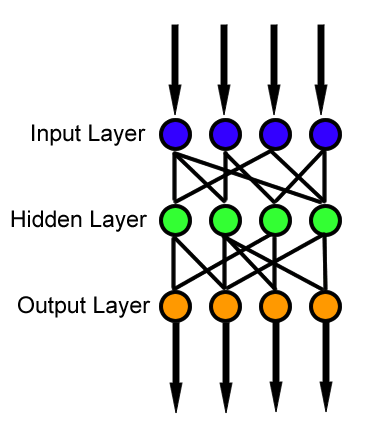
\includegraphics[height=6cm,keepaspectratio=true]
    {Feed_forward_neural_net.png}
    \caption{
        Feed forward neural network with 4 neurons each in every layer \cite{WikipediaEN_FeedForward_Network}.
    }
    \label{fig:Feed forward neural network}
\end{figure}

There are 3 layers in the figure and the extracted features of raw data will be sent through input layer. Each circle is a neuron with incoming lines as inputs and outgoing lines as outputs to next layer. Each line carries a weight and the input layer has no weights since it has no incoming lines. The output layer has no outgoing lines and will be used as final output. In this figure the hidden layers has 4 neurons which will have 4 weights and 1 bias variable for each of its neurons. At the beginning, the weights and bias variable are assigned with initial values. Each neuron also has a non-linear activation function such as sigmoid, hyperbolic tangent, rectifiers etc. Different activation functions poses different advantages and rectifiers are used common. This activation function will help the neural network models to approximate any non-linear function. The output layer can use a transformation function such as softmax to convert values to represent a discrete probability distribution. In this figure, 4 neurons are used and so it refers to 4 labels and this system classifies the input into one of the labels.

Training is an essential part of learning and like many supervised algorithms a loss function is used to compute the error for the estimated output against the actual output. Some of the loss functions that could be used are hinge (binary and multiclass), log loss, categorical cross-entropy loss etc. The gradient of the errors are calculated and propagated back to compute with respect to weights and bias. The values of the weights and bias are adjusted with respect to the gradient and a learning parameter. Typically a random batch of input are selected and parameters are applied and the output is computed. The average loss is computed for that batch and the parameters are reassigned. This optimization technique is called stochastic gradient descent \cite{Bottou2012} and other techniques available are Nesterov Momentum, AdaGrad etc. The overfitting in neural networks can be minimized by using regularization techniques such as L\textsubscript{2} regularization and dropout\cite{Hinton2012}. The L\textsubscript{2} regularization works by adding a squared penalty on parameters with respect to the function being minimized. The dropout works by randomly ignoring half of neurons in a networks or in every specific layer in each batch and corrects the error only using the parameters of other half of neurons. This helps to prevent the network from relying on only specific weights. 

Feedforward networks works very well on structured input data and incase of text data the input is arbitrary. Techniques such as continuous bag of words can be used to convert the arbitrary input into fixed length but it will lose the order of the text which is crucial. Convolutional neural network (CNN) \cite{Bengio1997} are good in capturing the local characteristics of data irrespective of its position. In this, a non linear function is applied to every k-word sliding window and captures the important characteristics of the word in that window. All the important characteristics from each window are combined by either taking maximum or average value from each window. This captures the important characteristics of sentence irrespective of their location. But yet the support for order is restricted only to local patterns and fails to recognize orders that are far apart in the sequence.

Recurrent neural networks (RNN) accepts arbitrary size input, pays attention to the structure and considers the long dependencies \cite{Elman}. RNN takes input as an ordered list of input vectors such as x\textsubscript{i:j} with initial state vector h\textsubscript{0} and returns an ordered list of state vectors h\textsubscript{1},...,h\textsubscript{n} as well as an ordered list of output vectors o\textsubscript{1},...,o\textsubscript{n}. At time step t, RNN takes input a state vector h\textsubscript{t-1}, an input vector x\textsubscript{t} and outputs a new state vector h\textsubscript{t} as shown in the figure. The outputted state vector is used as input state vector at the next time step. The same weights for input, state and output vectors are used in each and every time step.   


%RNN - architecture, how does it support the sequence, (Elman, 1990) 
%Back Propagation through time (BPTT) - (Werbos, 1990) \cite{Werbos1990}
%Long distance dependencies - LSTM and GRU (Hochreiter and Schmidhuber 1997) and (Cho et al.)
%(did not find the citation for GRU) \cite{Hochreiter1997}
%Recursive Neural Networks - for syntactic structure (trees ) (pollack 1990; socher, manning and ng 2010) \cite{Pollack1990} \cite{Socher}

\begin{figure}[htpb]
    \centering
    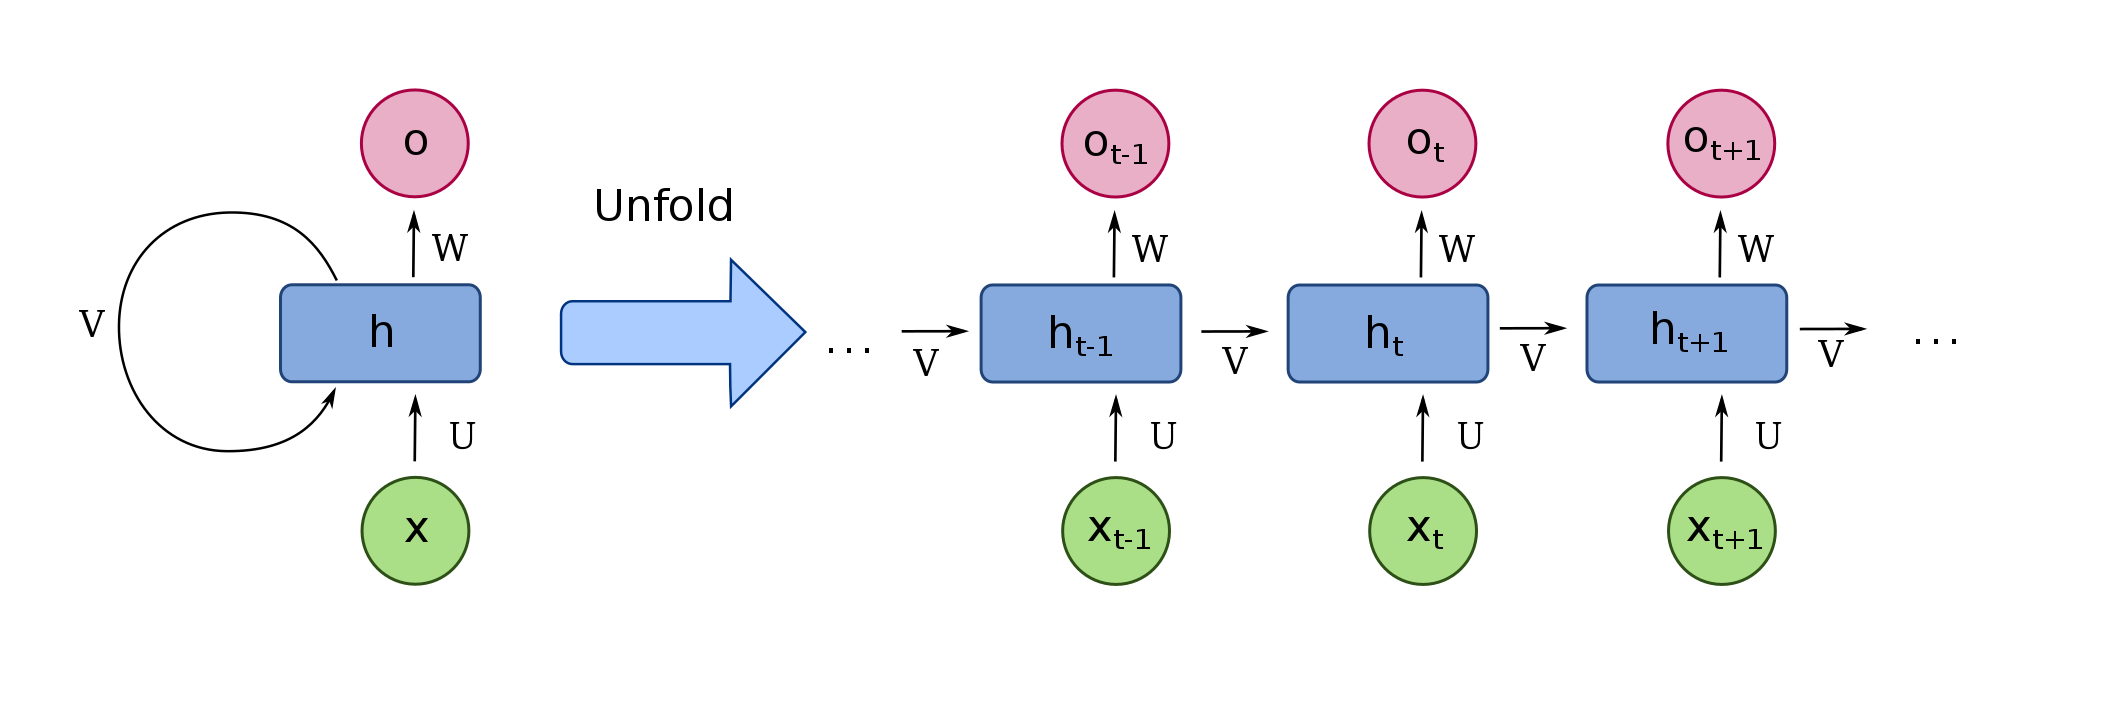
\includegraphics[width=\textwidth,height=6cm,keepaspectratio=true]
    {Recurrent_neural_network_unfold.png}
    \caption{
        A basic example of RNN architecture \cite{WikipediaEN_RNN_unfold}.
    }
    \label{fig:A basic RNN architecture}
\end{figure}

To train RNN, the network is unrolled for the given input sequence and the loss function uses these nodes to compute the error and propagate backward depending on the application \cite{Werbos1990}. While training, the error gradients might vanish or explode especially when dealing with RNNs. The gradient explosion can be handled by clipping the gradient when it goes beyond the threshold. LSTM networks \cite{Hochreiter1997} solves vanishing gradient problem by introducing memory cells which remembers gradients across time steps. The memory cells are controlled by mathematical functions which simulate logical gates called gating components. At each time step, a decision is made by gating components on how much of current content of memory cell and new input should be retained. 


\section{Approach}

Deep learning systems are giving better results in building intellectual systems nowadays.\cite{Goldberg2016} The results achieved in applications such as Autonomous car driving, playing chess are almost equivalent to the skillsets of a human. There are different neural network models exists such as Feed Forward, Convolutional, Recurrent Neural Network models. Wikipedia contains a lot of articles and each articles contains text. Text is a sequence data where as position of words in it is dependent on the other. Recurrent Neural Networks bring out best results in many applications involving text data such as machine translation, super tagging.

Every article or sentence in wikipedia can be fetched and inputted to the neural network as truthy value. But we lack false values. We need to use a semi supervised technique where in extraction of falsy values need to be carried out automatically. This is one of the challenges of this master thesis. 

Some of the ideas in place are
1) Extract the articles and sentences from many of these fact checkers websites and use the ones which are labelled as false values. We need to make sure that they are opposites of sentences in wikipedia.
2) Build sentences which are opposite of sentences in wikipedia by using GLOVE technique or construct negative sentences. 
3) Build sentences which are opposite of sentences in wikipedia by looking a semantic web representations. Word embeddings can be used to replace the verb opposites 

The size of the article in wikipedia are long and arbitrary and RNN will face gradient diminishing problems. The long distance dependencies will be missed out and hence different configurations of the neural network should be used and compared 
1) Different layers
2) Single/Multiple LSTM or GRU units
3) Usage of one hot vector vs word embeddings. The creation of word embeddings need to be thought through. It would be a good idea to do it from either wikipedia itself or from pre-trained word embeddiings


Recently convolutional neural network which character level input is giving out better results for some applications and this configuraiton should also be tried out.

%Deep learning - using RNN network architecture for sequential models
%One hot representation or word vector
%https://www.mendeley.com/viewer/?fileId=3eea8d80-58e9-51f5-5b45-945420ba7577&documentId=a45b2cdb-dae1-3d54-8d47-395580293df7

%Usage of LSTM - to support long range dependencies
%Wordvectors? 
%Language modeling? - Based on the probability of occurrence - we can predict how likely the sentence can occur or predict the next word. Given a news - predict how likely it can happen. But this may  not give a good result - so, can be used as a baseline

%Some research questions are

%What would be the best word vector representation for this problem - how do we prepare it? - have to generalize it
%How do we create negative examples? What is the best way to do it for this kind of problem?
%What lies can be detected effectively? This will explain what level of information is updated in wikipedia in each domain - constructing the dataset would be tricky. Can look at ways how to construct datasets based on the domain


\color{red}
Overall the things to do listed here are less and need to be appended more. Most of the stuff will be done in the prototyping phase itself . Will have to think about including ideas such as using DBPedia or any semantic database which is precisely expressed, Usage of any specific word embeddings or think of some other NLP techniques which could be used. Will have to be concrete at the same time. Need not be very strict - such as things specified here when both the parties agreed can be changed. Add new stuff, delete some other stuff and change or take a new direction. Things are possible but be reasonable

At some point when the methodology is specified, there should be a paragraph explaining about why these methodolgy are important and how different it is from the work done in related section. It can go here or somewhere in the introduction section
\color{black}

% ----------------------------------------------------------------------------
\section{Evaluation}

The training, evaluation and test dataset needs to be curated. 

More or less equal data should be present for each bin such as facts and lies.

Extract sentence from wikipedia and give it as it is.

Distort the sentence by swapping and give it.

Construct good facts and lies outside - a proper labelled dataset and see how it works.

Use the dataset provided by researches indicated in related work section.

Look for already curated community wide popular datasets for fake news.

Have a baseline.

Compare each configuration against baseline and measure the accuracy, time taken. If the curated dataset has many groups of varying complexity then state the results groupwise


\color{red}
The structure is good. Might have to explain the metrics listed. Why it is chosen and why it is important. Let us say for e.g. if we choose our implementation only aiming speed then time taken is important
\color{black}

\newpage

% ----------------------------------------------------------------------------
\section{Organizational matters}

\begin{tabbing}
Duration of work: \hspace{1.1cm} \= \StartDate{} -- \EndDate{}\\
\vspace{0.5ex}Candidate:	\> \myName{}\\
\vspace{0.5ex}E-Mail:	\> \emailID{}\\
\vspace{0.5ex}Student number: \> \matriculationID{}\\
\vspace{0.5ex}Primary supervisor: \> \expert{}\\
Supervisor: \> \supervisor{}\\
Secondary supervisor: \> \secondSupervisor{}\\
\end{tabbing}

% ----------------------------------------------------------------------------

\section{Time schedule}

\begin{itemize}
	\item Introduction and Literature: 01-May-2018 – 30-June-2018
	\item Initial Phase: 01-July-2018 – 15-Sep-2018
	\begin{itemize}
		\item Prototyping: 01-July-2018 – 30-July-2018
		\item Implementing ML Pipeline: 01-Aug-2018 – 15-Aug-2018
        \item Baseline Implementation: 16-Aug-2018 – 30-Aug-2018
        \item Testing and refining: 01-Sep-2018 – 15-Sep-2018
	\end{itemize}
	\item Development Phase: 16-Sep-2018 – 30-Nov-2018
	\begin{itemize}
		\item Prototyping: 01-July-2018 – 30-July-2018
		\item Implementing ML Pipeline: 01-Aug-2018 – 15-Aug-2018
        \item Baseline Implementation: 16-Aug-2018 – 30-Aug-2018
        \item Testing and refining: 01-Sep-2018 – 15-Sep-2018
	\end{itemize}
	\item Final Phase: 01-Dec-2018 – 30-Dec-2018
	\begin{itemize}
	 	\item Comprehend Benchamark results: 01-Dec-2018 – 15-Dec-2018
		\item Revision: 08-Dec-2018 – 22-Dec-2018
		\item Thesis report: 01-Dec-2018 – 30-Dec-2018
	\end{itemize}
\end{itemize}


% ----------------------------------------------------------------------------
\bibliographystyle{alpha}
\newpage
\bibliography{bib}
\newpage
% ----------------------------------------------------------------------------
\section{Signatures}

\vspace{3cm}
\begin{tabular}{ccc}
  --------------------------------------------------- &  & ---------------------------------------------------\\
  \myName{} &  & \expert{}  \\ \vspace{3cm}
   &  &   \\
  --------------------------------------------------- &  & ---------------------------------------------------\\
  \supervisor{} &  & \secondSupervisor{}  \\ \vspace{3cm}
   &  &   \\
\end{tabular}

\newpage
% ----------------------------------------------------------------------------
\section{Declaration of Authorship}
I hereby declare that the thesis submitted is my own unaided work. All direct or indirect sources used are acknowledged as references.

I am aware that the thesis in digital form can be examined for the use of unauthorized aid and in order to determine whether the thesis as a whole or parts incorporated in it may be deemed as plagiarism. For the comparison of my work with existing sources I agree that it shall be entered in a database where it shall also remain after examination, to enable comparison with future theses submitted. Further rights of reproduction and usage, however, are not granted here.

This paper was not previously presented to another examination board and has not been published.

\vspace{3cm}
\begin{tabular}{ccc}

  Koblenz, on \today &  &  \\
     &  & ---------------------------------------------------\\
   &  & \myName{}  \\
\end{tabular}



\end{document}









